\section{Digital image representations}
As with everything else that is stored on a computer, images are encoded as a sequence of bits.
RGB images are popular representations, where each pixel is stored as three sequential bytes representing each color.
This representation is very intuitive and easy to understand, but other representations might be more suitable for certain applications.

\section{Luminance and chrominance}
In many use cases, each pixel's luminance (brightness) contains more helpful information than its chrominance (color), and separating these two components is beneficial.
This is relevant for visualization, as the human eye is more sensitive to changes in luminance than chrominance  \cite{lambWhyRodsCones2016}.
It can also apply to computer vision applications, where Lucas-Kanade is an example of an optical flow algorithm that only uses the luminance component \cite{lucasIterativeImageRegistration1981}.

YCbCr
\footnote{In the computer industry, the term YUV is widely used to refer to colorspaces that are encoded using YCbCr.}
is a popular color format where the Y component represents the luminance of the pixel, while the Cb and Cr components represent the blue-difference and red-difference chrominance information respectively, as depicted in Figure \ref{fig:ycbcr_example}.

\begin{figure}[H]
    \centering
    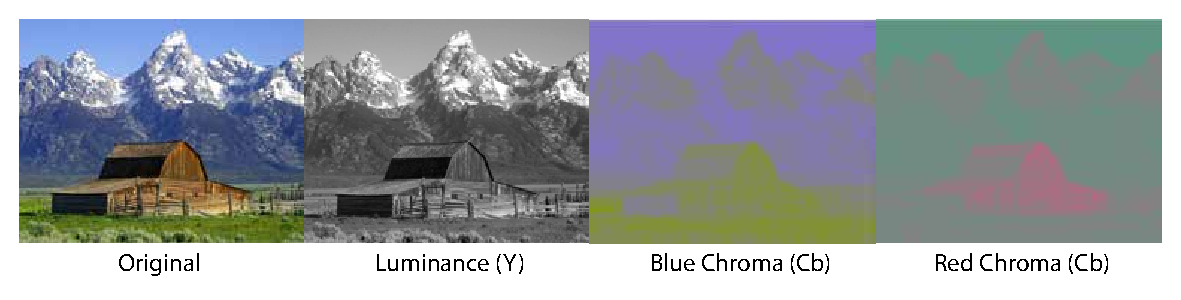
\includegraphics[width=\textwidth]{figures/debayer/YCbCr_example.pdf}
    \caption{Visualization of channels in a YCbCr image \cite{photoEnglishJohnMoulton2004}.}
    \label{fig:ycbcr_example}
\end{figure}

\subsubsection{Chroma subsampling}
Chroma subsampling is a technique that involves sampling the chrominance components (Cb and Cr) at a lower resolution than the luminance component (Y), as depicted in Figure \ref{fig:chroma_subsampling}.
A commonly used subsampling scheme is 4:2:0, where the chrominance components are sampled at half the resolution of the luminance component in both the horizontal and vertical directions \cite{ChromaSubsampling2023}.

During the process of debayering, redundant information is generated as each pixel in the output image contains three color channels, compared to only one in the raw Bayer image.
With this redundancy it is reasonable to perform chroma subsampling as the luminance component is sampled at every pixel, while a group of four pixels is required to obtain color information

\begin{figure}[H]
    \centering
    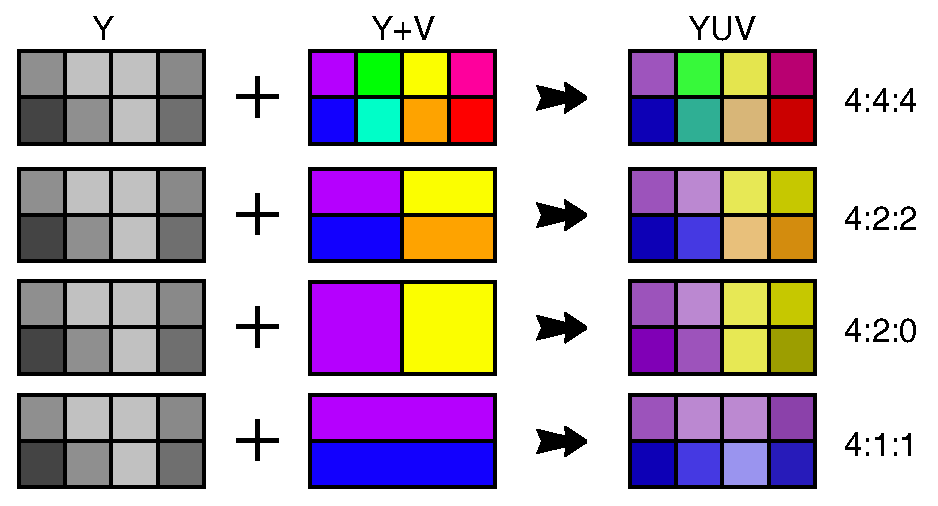
\includegraphics[width=.6\textwidth]{figures/debayer/chroma_subsampling.pdf}
    \caption{Chroma subsampling \cite{stevo-88EnglishMostWidely2010}.}
    \label{fig:chroma_subsampling}
\end{figure}


\subsection{Analog legacy}
It is important to note that certain color formats have their origins in the analog signal era.
One notable example is the BT.601 color format, a variant of YCbCr.
In this format, the Y component is represented by values ranging from 16 to 235, while the Cb and Cr components range from 16 to 240 \cite{YCbCr2023}.
The additional headroom and foot room within the byte is specifically allocated to accommodate transient signals, such as filter overshoots, and prevent undesirable effects like clipping \cite{Rec6012023}.
By reserving these values, the color representation remains within acceptable limits even when unexpected analog signal fluctuations occur.


\section{Interleved, Planar and Semi-Planar Packaging}
There are three main ways to store the color channels in memory, interleaved, planar and semi-planar \cite{baranYUVFormats2018}.
In interleaved formats, the color channels are stored in sequence, i.e.
$R_1 G_1 B_1 R_2 G_2 B_2 R_3 G_3 B_3$.
In planar formats, the color channels are stored in separate arrays, i.e.
$R_1 R_2 R_3 B_1 B_3 B_2 G_1 G_2 G_3$.
Semi-planar formats are a mix of the two where some channels are interleaved, and some are planar, i.e.
$R_1 R_2 R_3 G_1 B_1 G_2 B_2 G_3 B_3$.
The reson one might be preferred over the other is to optimize for memory locality.
For instance, if you are performing per-bit operations, having the bits of the same color channel next to each other is beneficial.

\begin{figure}[H]
    \centering
    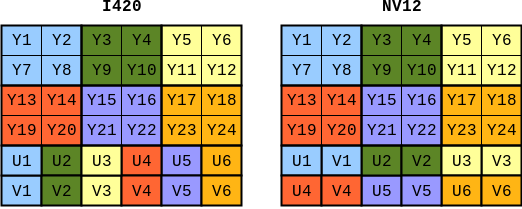
\includegraphics[width=.8\textwidth]{figures/debayer/YUV_packaging.png}
    \caption{Visualization of I420 and NV12, two popular YUV 4:2:0 formats with planar and semi-planar packaging respectively \cite{baranYUVFormats2018}.}
    \label{fig:image_packaging}
\end{figure}

\subsection{Bit depth and packaging}
A final important property of image formats is the bit depth, i.e.
how many bits are used to represent each pixel, and how the bits are stored.
Most images use a single byte (8 bits) for each color channel, but higher bit depths offer better color fidelity and dynamic range.
If the number of bits is not divisible by 8, like for 10-bit images, the most space-efficient way to store and send them is to pack them into 8-bit bytes, i.e.
four 10-bit values are stored in 5 bytes.
However, as most \glspl{alu} does not support 10-bit operations, padding to the nearest full byte is better for computations.